\documentclass[1p]{elsarticle_modified}
%\bibliographystyle{elsarticle-num}

%\usepackage[colorlinks]{hyperref}
%\usepackage{abbrmath_seonhwa} %\Abb, \Ascr, \Acal ,\Abf, \Afrak
\usepackage{amsfonts}
\usepackage{amssymb}
\usepackage{amsmath}
\usepackage{amsthm}
\usepackage{scalefnt}
\usepackage{amsbsy}
\usepackage{kotex}
\usepackage{caption}
\usepackage{subfig}
\usepackage{color}
\usepackage{graphicx}
\usepackage{xcolor} %% white, black, red, green, blue, cyan, magenta, yellow
\usepackage{float}
\usepackage{setspace}
\usepackage{hyperref}

\usepackage{tikz}
\usetikzlibrary{arrows}

\usepackage{multirow}
\usepackage{array} % fixed length table
\usepackage{hhline}

%%%%%%%%%%%%%%%%%%%%%
\makeatletter
\renewcommand*\env@matrix[1][\arraystretch]{%
	\edef\arraystretch{#1}%
	\hskip -\arraycolsep
	\let\@ifnextchar\new@ifnextchar
	\array{*\c@MaxMatrixCols c}}
\makeatother %https://tex.stackexchange.com/questions/14071/how-can-i-increase-the-line-spacing-in-a-matrix
%%%%%%%%%%%%%%%

\usepackage[normalem]{ulem}

\newcommand{\msout}[1]{\ifmmode\text{\sout{\ensuremath{#1}}}\else\sout{#1}\fi}
%SOURCE: \msout is \stkout macro in https://tex.stackexchange.com/questions/20609/strikeout-in-math-mode

\newcommand{\cancel}[1]{
	\ifmmode
	{\color{red}\msout{#1}}
	\else
	{\color{red}\sout{#1}}
	\fi
}

\newcommand{\add}[1]{
	{\color{blue}\uwave{#1}}
}

\newcommand{\replace}[2]{
	\ifmmode
	{\color{red}\msout{#1}}{\color{blue}\uwave{#2}}
	\else
	{\color{red}\sout{#1}}{\color{blue}\uwave{#2}}
	\fi
}

\newcommand{\Sol}{\mathcal{S}} %segment
\newcommand{\D}{D} %diagram
\newcommand{\A}{\mathcal{A}} %arc


%%%%%%%%%%%%%%%%%%%%%%%%%%%%%5 test

\def\sl{\operatorname{\textup{SL}}(2,\Cbb)}
\def\psl{\operatorname{\textup{PSL}}(2,\Cbb)}
\def\quan{\mkern 1mu \triangleright \mkern 1mu}

\theoremstyle{definition}
\newtheorem{thm}{Theorem}[section]
\newtheorem{prop}[thm]{Proposition}
\newtheorem{lem}[thm]{Lemma}
\newtheorem{ques}[thm]{Question}
\newtheorem{cor}[thm]{Corollary}
\newtheorem{defn}[thm]{Definition}
\newtheorem{exam}[thm]{Example}
\newtheorem{rmk}[thm]{Remark}
\newtheorem{alg}[thm]{Algorithm}

\newcommand{\I}{\sqrt{-1}}
\begin{document}

%\begin{frontmatter}
%
%\title{Boundary parabolic representations of knots up to 8 crossings}
%
%%% Group authors per affiliation:
%\author{Yunhi Cho} 
%\address{Department of Mathematics, University of Seoul, Seoul, Korea}
%\ead{yhcho@uos.ac.kr}
%
%
%\author{Seonhwa Kim} %\fnref{s_kim}}
%\address{Center for Geometry and Physics, Institute for Basic Science, Pohang, 37673, Korea}
%\ead{ryeona17@ibs.re.kr}
%
%\author{Hyuk Kim}
%\address{Department of Mathematical Sciences, Seoul National University, Seoul 08826, Korea}
%\ead{hyukkim@snu.ac.kr}
%
%\author{Seokbeom Yoon}
%\address{Department of Mathematical Sciences, Seoul National University, Seoul, 08826,  Korea}
%\ead{sbyoon15@snu.ac.kr}
%
%\begin{abstract}
%We find all boundary parabolic representation of knots up to 8 crossings.
%
%\end{abstract}
%\begin{keyword}
%    \MSC[2010] 57M25 
%\end{keyword}
%
%\end{frontmatter}

%\linenumbers
%\tableofcontents
%
\newcommand\colored[1]{\textcolor{white}{\rule[-0.35ex]{0.8em}{1.4ex}}\kern-0.8em\color{red} #1}%
%\newcommand\colored[1]{\textcolor{white}{ #1}\kern-2.17ex	\textcolor{white}{ #1}\kern-1.81ex	\textcolor{white}{ #1}\kern-2.15ex\color{red}#1	}

{\Large $\underline{12n_{0295}~(K12n_{0295})}$}

\setlength{\tabcolsep}{10pt}
\renewcommand{\arraystretch}{1.6}
\vspace{1cm}\begin{tabular}{m{100pt}>{\centering\arraybackslash}m{274pt}}
\multirow{5}{120pt}{
	\centering
	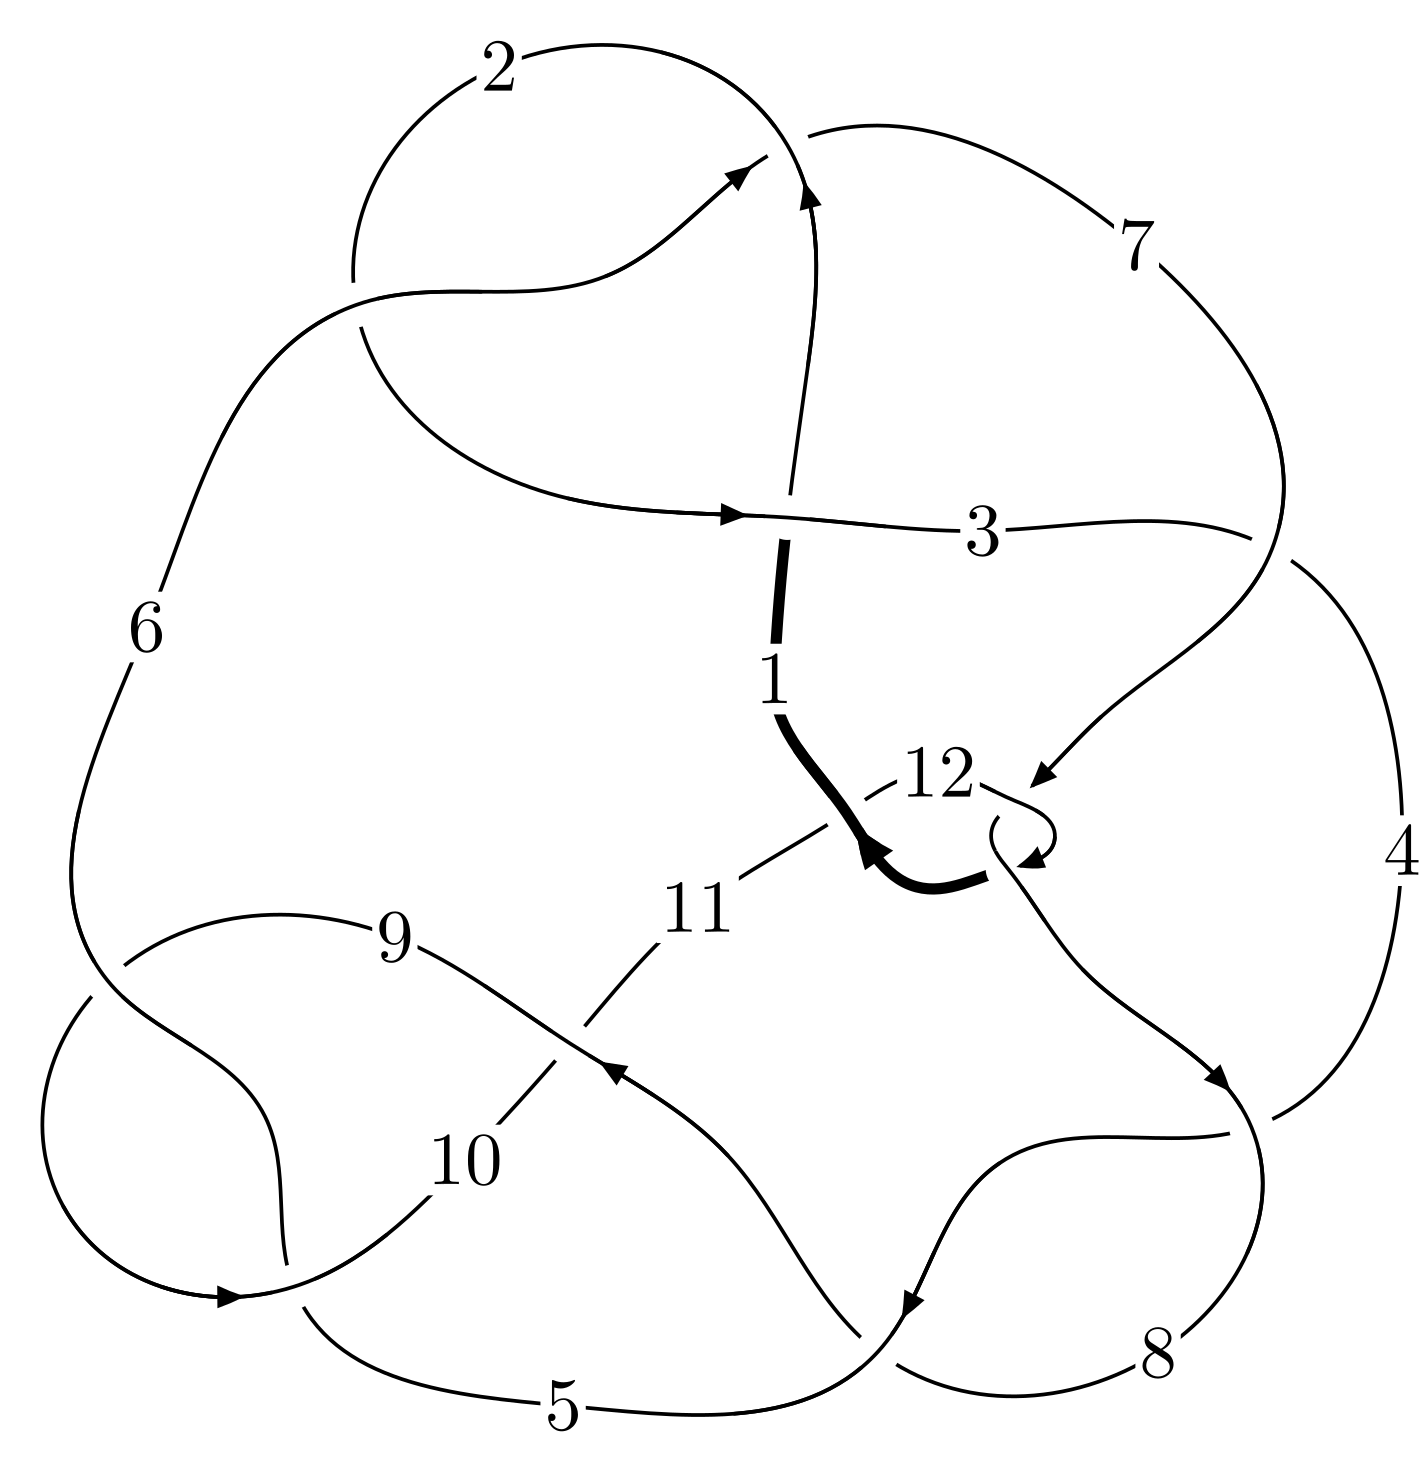
\includegraphics[width=112pt]{../../../GIT/diagram.site/Diagrams/png/2384_12n_0295.png}\\
\ \ \ A knot diagram\footnotemark}&
\allowdisplaybreaks
\textbf{Linearized knot diagam} \\
\cline{2-2}
 &
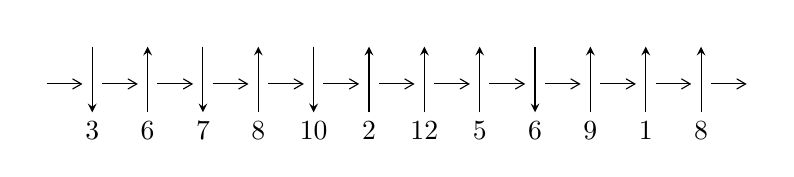
\begin{tikzpicture}[x=20pt, y=17pt]
	% nodes
	\node (C0) at (0, 0) {};
	\node (C1) at (1, 0) {};
	\node (C1U) at (1, +1) {};
	\node (C1D) at (1, -1) {3};

	\node (C2) at (2, 0) {};
	\node (C2U) at (2, +1) {};
	\node (C2D) at (2, -1) {6};

	\node (C3) at (3, 0) {};
	\node (C3U) at (3, +1) {};
	\node (C3D) at (3, -1) {7};

	\node (C4) at (4, 0) {};
	\node (C4U) at (4, +1) {};
	\node (C4D) at (4, -1) {8};

	\node (C5) at (5, 0) {};
	\node (C5U) at (5, +1) {};
	\node (C5D) at (5, -1) {10};

	\node (C6) at (6, 0) {};
	\node (C6U) at (6, +1) {};
	\node (C6D) at (6, -1) {2};

	\node (C7) at (7, 0) {};
	\node (C7U) at (7, +1) {};
	\node (C7D) at (7, -1) {12};

	\node (C8) at (8, 0) {};
	\node (C8U) at (8, +1) {};
	\node (C8D) at (8, -1) {5};

	\node (C9) at (9, 0) {};
	\node (C9U) at (9, +1) {};
	\node (C9D) at (9, -1) {6};

	\node (C10) at (10, 0) {};
	\node (C10U) at (10, +1) {};
	\node (C10D) at (10, -1) {9};

	\node (C11) at (11, 0) {};
	\node (C11U) at (11, +1) {};
	\node (C11D) at (11, -1) {1};

	\node (C12) at (12, 0) {};
	\node (C12U) at (12, +1) {};
	\node (C12D) at (12, -1) {8};
	\node (C13) at (13, 0) {};

	% arrows
	\draw[->,>={angle 60}]
	(C0) edge (C1) (C1) edge (C2) (C2) edge (C3) (C3) edge (C4) (C4) edge (C5) (C5) edge (C6) (C6) edge (C7) (C7) edge (C8) (C8) edge (C9) (C9) edge (C10) (C10) edge (C11) (C11) edge (C12) (C12) edge (C13) ;	\draw[->,>=stealth]
	(C1U) edge (C1D) (C2D) edge (C2U) (C3U) edge (C3D) (C4D) edge (C4U) (C5U) edge (C5D) (C6D) edge (C6U) (C7D) edge (C7U) (C8D) edge (C8U) (C9U) edge (C9D) (C10D) edge (C10U) (C11D) edge (C11U) (C12D) edge (C12U) ;
	\end{tikzpicture} \\
\hhline{~~} \\& 
\textbf{Solving Sequence} \\ \cline{2-2} 
 &
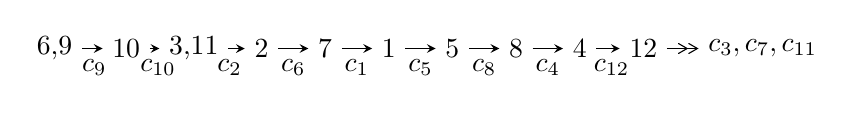
\begin{tikzpicture}[x=23pt, y=7pt]
	% node
	\node (A0) at (-1/8, 0) {6,9};
	\node (A1) at (1, 0) {10};
	\node (A2) at (33/16, 0) {3,11};
	\node (A3) at (25/8, 0) {2};
	\node (A4) at (33/8, 0) {7};
	\node (A5) at (41/8, 0) {1};
	\node (A6) at (49/8, 0) {5};
	\node (A7) at (57/8, 0) {8};
	\node (A8) at (65/8, 0) {4};
	\node (A9) at (73/8, 0) {12};
	\node (C1) at (1/2, -1) {$c_{9}$};
	\node (C2) at (3/2, -1) {$c_{10}$};
	\node (C3) at (21/8, -1) {$c_{2}$};
	\node (C4) at (29/8, -1) {$c_{6}$};
	\node (C5) at (37/8, -1) {$c_{1}$};
	\node (C6) at (45/8, -1) {$c_{5}$};
	\node (C7) at (53/8, -1) {$c_{8}$};
	\node (C8) at (61/8, -1) {$c_{4}$};
	\node (C9) at (69/8, -1) {$c_{12}$};
	\node (A10) at (11, 0) {$c_{3},c_{7},c_{11}$};

	% edge
	\draw[->,>=stealth]	
	(A0) edge (A1) (A1) edge (A2) (A2) edge (A3) (A3) edge (A4) (A4) edge (A5) (A5) edge (A6) (A6) edge (A7) (A7) edge (A8) (A8) edge (A9) ;
	\draw[->>,>={angle 60}]	
	(A9) edge (A10);
\end{tikzpicture} \\ 

\end{tabular} \\

\footnotetext{
The image of knot diagram is generated by the software ``\textbf{Draw programme}" developed by Andrew Bartholomew(\url{http://www.layer8.co.uk/maths/draw/index.htm\#Running-draw}), where we modified some parts for our purpose(\url{https://github.com/CATsTAILs/LinksPainter}).
}\phantom \\ \newline 
\centering \textbf{Ideals for irreducible components\footnotemark of $X_{\text{par}}$} 
 
\begin{align*}
I^u_{1}&=\langle 
1.06469\times10^{32} u^{66}-1.40021\times10^{32} u^{65}+\cdots+2.98795\times10^{31} b-4.19610\times10^{32},\\
\phantom{I^u_{1}}&\phantom{= \langle  }-1.94960\times10^{31} u^{66}-3.90032\times10^{31} u^{65}+\cdots+2.98795\times10^{31} a-2.08028\times10^{32},\;u^{67}- u^{66}+\cdots-4 u+4\rangle \\
I^u_{2}&=\langle 
u^3 a- u^2 a+a u- u^2+b-2 a+u-1,\;u^3 a+2 a^2+2 a u- u^2-2,\;u^4+2 u^2+2\rangle \\
\\
I^v_{1}&=\langle 
a,\;b+v,\;v^2- v+1\rangle \\
\end{align*}
\raggedright * 3 irreducible components of $\dim_{\mathbb{C}}=0$, with total 77 representations.\\
\footnotetext{All coefficients of polynomials are rational numbers. But the coefficients are sometimes approximated in decimal forms when there is not enough margin.}
\newpage
\renewcommand{\arraystretch}{1}
\centering \section*{I. $I^u_{1}= \langle 1.06\times10^{32} u^{66}-1.40\times10^{32} u^{65}+\cdots+2.99\times10^{31} b-4.20\times10^{32},\;-1.95\times10^{31} u^{66}-3.90\times10^{31} u^{65}+\cdots+2.99\times10^{31} a-2.08\times10^{32},\;u^{67}- u^{66}+\cdots-4 u+4 \rangle$}
\flushleft \textbf{(i) Arc colorings}\\
\begin{tabular}{m{7pt} m{180pt} m{7pt} m{180pt} }
\flushright $a_{6}=$&$\begin{pmatrix}0\\u\end{pmatrix}$ \\
\flushright $a_{9}=$&$\begin{pmatrix}1\\0\end{pmatrix}$ \\
\flushright $a_{10}=$&$\begin{pmatrix}1\\u^2\end{pmatrix}$ \\
\flushright $a_{3}=$&$\begin{pmatrix}0.652488 u^{66}+1.30535 u^{65}+\cdots+3.13714 u+6.96225\\-3.56329 u^{66}+4.68621 u^{65}+\cdots-16.7518 u+14.0434\end{pmatrix}$ \\
\flushright $a_{11}=$&$\begin{pmatrix}u^2+1\\u^2\end{pmatrix}$ \\
\flushright $a_{2}=$&$\begin{pmatrix}0.652488 u^{66}+1.30535 u^{65}+\cdots+3.13714 u+6.96225\\-2.60763 u^{66}+2.64905 u^{65}+\cdots-11.5304 u+6.21206\end{pmatrix}$ \\
\flushright $a_{7}=$&$\begin{pmatrix}-3.25872 u^{66}+3.19768 u^{65}+\cdots-14.7929 u+8.57622\\2.29504 u^{66}-0.672961 u^{65}+\cdots+9.68506 u-2.51477\end{pmatrix}$ \\
\flushright $a_{1}=$&$\begin{pmatrix}0.0915661 u^{66}-1.99663 u^{65}+\cdots+2.63606 u-7.72366\\-4.93115 u^{66}+4.21632 u^{65}+\cdots-21.8384 u+11.2155\end{pmatrix}$ \\
\flushright $a_{5}=$&$\begin{pmatrix}u\\u^3+u\end{pmatrix}$ \\
\flushright $a_{8}=$&$\begin{pmatrix}u^4+u^2+1\\u^6+2 u^4+u^2\end{pmatrix}$ \\
\flushright $a_{4}=$&$\begin{pmatrix}- u^7-2 u^5-2 u^3\\- u^9-3 u^7-3 u^5+u\end{pmatrix}$ \\
\flushright $a_{12}=$&$\begin{pmatrix}0.709744 u^{66}-1.32832 u^{65}+\cdots+4.54050 u-3.81522\\-5.57978 u^{66}+5.85739 u^{65}+\cdots-26.2200 u+17.2657\end{pmatrix}$\\&\end{tabular}
\flushleft \textbf{(ii) Obstruction class $= -1$}\\~\\
\flushleft \textbf{(iii) Cusp Shapes $= 3.44470 u^{66}-8.34775 u^{65}+\cdots+29.7826 u-28.7599$}\\~\\
\newpage\renewcommand{\arraystretch}{1}
\flushleft \textbf{(iv) u-Polynomials at the component}\newline \\
\begin{tabular}{m{50pt}|m{274pt}}
Crossings & \hspace{64pt}u-Polynomials at each crossing \\
\hline $$\begin{aligned}c_{1}\end{aligned}$$&$\begin{aligned}
&u^{67}+38 u^{66}+\cdots-4 u-1
\end{aligned}$\\
\hline $$\begin{aligned}c_{2},c_{6}\end{aligned}$$&$\begin{aligned}
&u^{67}-2 u^{66}+\cdots+6 u-1
\end{aligned}$\\
\hline $$\begin{aligned}c_{3}\end{aligned}$$&$\begin{aligned}
&u^{67}+2 u^{66}+\cdots+734 u-173
\end{aligned}$\\
\hline $$\begin{aligned}c_{4},c_{8}\end{aligned}$$&$\begin{aligned}
&u^{67}- u^{66}+\cdots-52 u-548
\end{aligned}$\\
\hline $$\begin{aligned}c_{5},c_{9}\end{aligned}$$&$\begin{aligned}
&u^{67}+u^{66}+\cdots-4 u-4
\end{aligned}$\\
\hline $$\begin{aligned}c_{7},c_{12}\end{aligned}$$&$\begin{aligned}
&u^{67}-3 u^{66}+\cdots-15 u-13
\end{aligned}$\\
\hline $$\begin{aligned}c_{10}\end{aligned}$$&$\begin{aligned}
&u^{67}-31 u^{66}+\cdots-80 u+16
\end{aligned}$\\
\hline $$\begin{aligned}c_{11}\end{aligned}$$&$\begin{aligned}
&u^{67}-23 u^{66}+\cdots+3501 u-169
\end{aligned}$\\
\hline
\end{tabular}\\~\\
\newpage\renewcommand{\arraystretch}{1}
\flushleft \textbf{(v) Riley Polynomials at the component}\newline \\
\begin{tabular}{m{50pt}|m{274pt}}
Crossings & \hspace{64pt}Riley Polynomials at each crossing \\
\hline $$\begin{aligned}c_{1}\end{aligned}$$&$\begin{aligned}
&y^{67}-10 y^{66}+\cdots+84 y-1
\end{aligned}$\\
\hline $$\begin{aligned}c_{2},c_{6}\end{aligned}$$&$\begin{aligned}
&y^{67}+38 y^{66}+\cdots-4 y-1
\end{aligned}$\\
\hline $$\begin{aligned}c_{3}\end{aligned}$$&$\begin{aligned}
&y^{67}-58 y^{66}+\cdots-506856 y-29929
\end{aligned}$\\
\hline $$\begin{aligned}c_{4},c_{8}\end{aligned}$$&$\begin{aligned}
&y^{67}- y^{66}+\cdots-3289680 y-300304
\end{aligned}$\\
\hline $$\begin{aligned}c_{5},c_{9}\end{aligned}$$&$\begin{aligned}
&y^{67}+31 y^{66}+\cdots-80 y-16
\end{aligned}$\\
\hline $$\begin{aligned}c_{7},c_{12}\end{aligned}$$&$\begin{aligned}
&y^{67}-23 y^{66}+\cdots+3501 y-169
\end{aligned}$\\
\hline $$\begin{aligned}c_{10}\end{aligned}$$&$\begin{aligned}
&y^{67}+15 y^{66}+\cdots-3328 y-256
\end{aligned}$\\
\hline $$\begin{aligned}c_{11}\end{aligned}$$&$\begin{aligned}
&y^{67}+57 y^{66}+\cdots+203921 y-28561
\end{aligned}$\\
\hline
\end{tabular}\\~\\
\newpage\flushleft \textbf{(vi) Complex Volumes and Cusp Shapes}
$$\begin{array}{c|c|c}  
\text{Solutions to }I^u_{1}& \I (\text{vol} + \sqrt{-1}CS) & \text{Cusp shape}\\
 \hline 
\begin{aligned}
u &= -0.293686 + 0.958960 I \\
a &= -0.848658 - 0.410982 I \\
b &= -1.26966 - 0.89610 I\end{aligned}
 & \phantom{-}3.60658 - 1.32410 I & \phantom{-}10.41239 + 2.57758 I \\ \hline\begin{aligned}
u &= -0.293686 - 0.958960 I \\
a &= -0.848658 + 0.410982 I \\
b &= -1.26966 + 0.89610 I\end{aligned}
 & \phantom{-}3.60658 + 1.32410 I & \phantom{-}10.41239 - 2.57758 I \\ \hline\begin{aligned}
u &= -0.797556 + 0.595964 I \\
a &= \phantom{-}0.370623 - 1.314420 I \\
b &= -0.92158 - 2.06820 I\end{aligned}
 & -8.62301 + 6.67427 I & \phantom{-0.000000 } 0. - 5.42994 I \\ \hline\begin{aligned}
u &= -0.797556 - 0.595964 I \\
a &= \phantom{-}0.370623 + 1.314420 I \\
b &= -0.92158 + 2.06820 I\end{aligned}
 & -8.62301 - 6.67427 I & \phantom{-0.000000 -}0. + 5.42994 I \\ \hline\begin{aligned}
u &= \phantom{-}0.390812 + 0.942541 I \\
a &= -0.614053 - 0.918919 I \\
b &= -0.27889 - 2.74791 I\end{aligned}
 & \phantom{-}2.87894 - 3.62568 I & \phantom{-}4.00000 + 3.66828 I \\ \hline\begin{aligned}
u &= \phantom{-}0.390812 - 0.942541 I \\
a &= -0.614053 + 0.918919 I \\
b &= -0.27889 + 2.74791 I\end{aligned}
 & \phantom{-}2.87894 + 3.62568 I & \phantom{-}4.00000 - 3.66828 I \\ \hline\begin{aligned}
u &= \phantom{-}0.369468 + 0.905859 I \\
a &= -1.161530 + 0.100804 I \\
b &= \phantom{-}1.70277 + 0.10484 I\end{aligned}
 & \phantom{-}2.70033 + 0.62241 I & \phantom{-}6.92862 + 0. I\phantom{ +0.000000I} \\ \hline\begin{aligned}
u &= \phantom{-}0.369468 - 0.905859 I \\
a &= -1.161530 - 0.100804 I \\
b &= \phantom{-}1.70277 - 0.10484 I\end{aligned}
 & \phantom{-}2.70033 - 0.62241 I & \phantom{-}6.92862 + 0. I\phantom{ +0.000000I} \\ \hline\begin{aligned}
u &= -0.625687 + 0.815726 I \\
a &= -0.866747 + 0.736378 I \\
b &= \phantom{-}0.96397 + 1.91289 I\end{aligned}
 & -4.18859 + 2.44849 I & \phantom{-0.000000 } 0 \\ \hline\begin{aligned}
u &= -0.625687 - 0.815726 I \\
a &= -0.866747 - 0.736378 I \\
b &= \phantom{-}0.96397 - 1.91289 I\end{aligned}
 & -4.18859 - 2.44849 I & \phantom{-0.000000 } 0\\
 \hline 
 \end{array}$$\newpage$$\begin{array}{c|c|c}  
\text{Solutions to }I^u_{1}& \I (\text{vol} + \sqrt{-1}CS) & \text{Cusp shape}\\
 \hline 
\begin{aligned}
u &= \phantom{-}0.827360 + 0.500431 I \\
a &= -0.371421 - 1.339800 I \\
b &= \phantom{-}0.97307 - 1.82972 I\end{aligned}
 & -8.90984 + 0.43271 I & -1.022530 + 0.496680 I \\ \hline\begin{aligned}
u &= \phantom{-}0.827360 - 0.500431 I \\
a &= -0.371421 + 1.339800 I \\
b &= \phantom{-}0.97307 + 1.82972 I\end{aligned}
 & -8.90984 - 0.43271 I & -1.022530 - 0.496680 I \\ \hline\begin{aligned}
u &= -0.828153 + 0.492617 I \\
a &= -1.081770 + 0.896752 I \\
b &= \phantom{-}1.05437 + 1.68616 I\end{aligned}
 & -8.86607 - 3.17955 I & -0.988573 + 0.950602 I \\ \hline\begin{aligned}
u &= -0.828153 - 0.492617 I \\
a &= -1.081770 - 0.896752 I \\
b &= \phantom{-}1.05437 - 1.68616 I\end{aligned}
 & -8.86607 + 3.17955 I & -0.988573 - 0.950602 I \\ \hline\begin{aligned}
u &= \phantom{-}0.773593 + 0.535367 I \\
a &= \phantom{-}0.820590 - 0.525886 I \\
b &= \phantom{-}0.506080 + 0.187810 I\end{aligned}
 & -4.83958 - 1.65195 I & \phantom{-}2.33033 + 2.39714 I \\ \hline\begin{aligned}
u &= \phantom{-}0.773593 - 0.535367 I \\
a &= \phantom{-}0.820590 + 0.525886 I \\
b &= \phantom{-}0.506080 - 0.187810 I\end{aligned}
 & -4.83958 + 1.65195 I & \phantom{-}2.33033 - 2.39714 I \\ \hline\begin{aligned}
u &= \phantom{-}0.846926 + 0.407345 I \\
a &= \phantom{-}1.10299 + 0.93182 I \\
b &= -1.17325 + 1.47521 I\end{aligned}
 & -7.51011 + 10.16540 I & \phantom{-}0.84901 - 5.51887 I \\ \hline\begin{aligned}
u &= \phantom{-}0.846926 - 0.407345 I \\
a &= \phantom{-}1.10299 - 0.93182 I \\
b &= -1.17325 - 1.47521 I\end{aligned}
 & -7.51011 - 10.16540 I & \phantom{-}0.84901 + 5.51887 I \\ \hline\begin{aligned}
u &= -0.808297 + 0.434822 I \\
a &= -0.798749 - 0.636743 I \\
b &= -0.374659 + 0.223488 I\end{aligned}
 & -4.26028 - 4.81071 I & \phantom{-}3.21364 + 2.49973 I \\ \hline\begin{aligned}
u &= -0.808297 - 0.434822 I \\
a &= -0.798749 + 0.636743 I \\
b &= -0.374659 - 0.223488 I\end{aligned}
 & -4.26028 + 4.81071 I & \phantom{-}3.21364 - 2.49973 I\\
 \hline 
 \end{array}$$\newpage$$\begin{array}{c|c|c}  
\text{Solutions to }I^u_{1}& \I (\text{vol} + \sqrt{-1}CS) & \text{Cusp shape}\\
 \hline 
\begin{aligned}
u &= -0.393391 + 1.042260 I \\
a &= -0.204574 + 0.462109 I \\
b &= -0.204935 - 0.456540 I\end{aligned}
 & \phantom{-}4.35771 + 3.46092 I & \phantom{-0.000000 } 0 \\ \hline\begin{aligned}
u &= -0.393391 - 1.042260 I \\
a &= -0.204574 - 0.462109 I \\
b &= -0.204935 + 0.456540 I\end{aligned}
 & \phantom{-}4.35771 - 3.46092 I & \phantom{-0.000000 } 0 \\ \hline\begin{aligned}
u &= -0.102031 + 1.124100 I \\
a &= -0.074288 + 0.720806 I \\
b &= -0.252101 + 1.022590 I\end{aligned}
 & \phantom{-}1.05983 - 2.64924 I & \phantom{-0.000000 } 0 \\ \hline\begin{aligned}
u &= -0.102031 - 1.124100 I \\
a &= -0.074288 - 0.720806 I \\
b &= -0.252101 - 1.022590 I\end{aligned}
 & \phantom{-}1.05983 + 2.64924 I & \phantom{-0.000000 } 0 \\ \hline\begin{aligned}
u &= \phantom{-}0.499688 + 1.012210 I \\
a &= \phantom{-}0.890259 - 0.218223 I \\
b &= \phantom{-}0.757089 - 0.307916 I\end{aligned}
 & \phantom{-}1.97793 - 2.12988 I & \phantom{-0.000000 } 0 \\ \hline\begin{aligned}
u &= \phantom{-}0.499688 - 1.012210 I \\
a &= \phantom{-}0.890259 + 0.218223 I \\
b &= \phantom{-}0.757089 + 0.307916 I\end{aligned}
 & \phantom{-}1.97793 + 2.12988 I & \phantom{-0.000000 } 0 \\ \hline\begin{aligned}
u &= \phantom{-}0.548320 + 0.997805 I \\
a &= \phantom{-}0.696251 + 0.717636 I \\
b &= -2.01408 + 2.32374 I\end{aligned}
 & \phantom{-}1.30273 - 5.96282 I & \phantom{-0.000000 } 0 \\ \hline\begin{aligned}
u &= \phantom{-}0.548320 - 0.997805 I \\
a &= \phantom{-}0.696251 - 0.717636 I \\
b &= -2.01408 - 2.32374 I\end{aligned}
 & \phantom{-}1.30273 + 5.96282 I & \phantom{-0.000000 } 0 \\ \hline\begin{aligned}
u &= -0.003645 + 1.165290 I \\
a &= \phantom{-}1.040750 + 0.337542 I \\
b &= -0.279122 + 0.832538 I\end{aligned}
 & -2.94562 - 1.34587 I & \phantom{-0.000000 } 0 \\ \hline\begin{aligned}
u &= -0.003645 - 1.165290 I \\
a &= \phantom{-}1.040750 - 0.337542 I \\
b &= -0.279122 - 0.832538 I\end{aligned}
 & -2.94562 + 1.34587 I & \phantom{-0.000000 } 0\\
 \hline 
 \end{array}$$\newpage$$\begin{array}{c|c|c}  
\text{Solutions to }I^u_{1}& \I (\text{vol} + \sqrt{-1}CS) & \text{Cusp shape}\\
 \hline 
\begin{aligned}
u &= \phantom{-}0.298119 + 0.774004 I \\
a &= \phantom{-}0.239287 + 0.602551 I \\
b &= -0.040611 + 0.560440 I\end{aligned}
 & \phantom{-}0.401806 - 1.265690 I & \phantom{-}4.47035 + 5.10756 I \\ \hline\begin{aligned}
u &= \phantom{-}0.298119 - 0.774004 I \\
a &= \phantom{-}0.239287 - 0.602551 I \\
b &= -0.040611 - 0.560440 I\end{aligned}
 & \phantom{-}0.401806 + 1.265690 I & \phantom{-}4.47035 - 5.10756 I \\ \hline\begin{aligned}
u &= -0.545451 + 1.036140 I \\
a &= \phantom{-}0.346086 - 0.872759 I \\
b &= -0.02443 - 2.31994 I\end{aligned}
 & \phantom{-}1.87665 + 7.41999 I & \phantom{-0.000000 } 0 \\ \hline\begin{aligned}
u &= -0.545451 - 1.036140 I \\
a &= \phantom{-}0.346086 + 0.872759 I \\
b &= -0.02443 + 2.31994 I\end{aligned}
 & \phantom{-}1.87665 - 7.41999 I & \phantom{-0.000000 } 0 \\ \hline\begin{aligned}
u &= -0.414664 + 1.113320 I \\
a &= -0.322911 - 0.117417 I \\
b &= -0.009462 - 1.064340 I\end{aligned}
 & \phantom{-}4.31530 + 3.66992 I & \phantom{-0.000000 } 0 \\ \hline\begin{aligned}
u &= -0.414664 - 1.113320 I \\
a &= -0.322911 + 0.117417 I \\
b &= -0.009462 + 1.064340 I\end{aligned}
 & \phantom{-}4.31530 - 3.66992 I & \phantom{-0.000000 } 0 \\ \hline\begin{aligned}
u &= \phantom{-}0.563544 + 0.577917 I \\
a &= \phantom{-}1.109400 + 0.643464 I \\
b &= -0.66998 + 2.28277 I\end{aligned}
 & \phantom{-}0.05661 + 1.47287 I & -0.156482 - 0.461455 I \\ \hline\begin{aligned}
u &= \phantom{-}0.563544 - 0.577917 I \\
a &= \phantom{-}1.109400 - 0.643464 I \\
b &= -0.66998 - 2.28277 I\end{aligned}
 & \phantom{-}0.05661 - 1.47287 I & -0.156482 + 0.461455 I \\ \hline\begin{aligned}
u &= \phantom{-}0.123549 + 1.190490 I \\
a &= -1.043430 + 0.330545 I \\
b &= \phantom{-}0.286253 + 1.175820 I\end{aligned}
 & -2.02431 + 7.56304 I & \phantom{-0.000000 } 0 \\ \hline\begin{aligned}
u &= \phantom{-}0.123549 - 1.190490 I \\
a &= -1.043430 - 0.330545 I \\
b &= \phantom{-}0.286253 - 1.175820 I\end{aligned}
 & -2.02431 - 7.56304 I & \phantom{-0.000000 } 0\\
 \hline 
 \end{array}$$\newpage$$\begin{array}{c|c|c}  
\text{Solutions to }I^u_{1}& \I (\text{vol} + \sqrt{-1}CS) & \text{Cusp shape}\\
 \hline 
\begin{aligned}
u &= -0.670786 + 1.018810 I \\
a &= \phantom{-}1.078320 - 0.268018 I \\
b &= -0.60969 - 1.60312 I\end{aligned}
 & -7.35703 - 1.17039 I & \phantom{-0.000000 } 0 \\ \hline\begin{aligned}
u &= -0.670786 - 1.018810 I \\
a &= \phantom{-}1.078320 + 0.268018 I \\
b &= -0.60969 + 1.60312 I\end{aligned}
 & -7.35703 + 1.17039 I & \phantom{-0.000000 } 0 \\ \hline\begin{aligned}
u &= \phantom{-}0.431796 + 1.142180 I \\
a &= \phantom{-}0.842437 - 0.007900 I \\
b &= \phantom{-}0.311709 - 0.277350 I\end{aligned}
 & \phantom{-}2.39569 - 1.20414 I & \phantom{-0.000000 } 0 \\ \hline\begin{aligned}
u &= \phantom{-}0.431796 - 1.142180 I \\
a &= \phantom{-}0.842437 + 0.007900 I \\
b &= \phantom{-}0.311709 + 0.277350 I\end{aligned}
 & \phantom{-}2.39569 + 1.20414 I & \phantom{-0.000000 } 0 \\ \hline\begin{aligned}
u &= \phantom{-}0.632532 + 1.049100 I \\
a &= -0.410549 + 0.627513 I \\
b &= -1.004620 + 0.513716 I\end{aligned}
 & -3.30409 - 3.65847 I & \phantom{-0.000000 } 0 \\ \hline\begin{aligned}
u &= \phantom{-}0.632532 - 1.049100 I \\
a &= -0.410549 - 0.627513 I \\
b &= -1.004620 - 0.513716 I\end{aligned}
 & -3.30409 + 3.65847 I & \phantom{-0.000000 } 0 \\ \hline\begin{aligned}
u &= -0.491913 + 1.123810 I \\
a &= \phantom{-}0.487065 - 0.297919 I \\
b &= \phantom{-}0.64193 - 2.20537 I\end{aligned}
 & \phantom{-}3.73381 + 3.87247 I & \phantom{-0.000000 } 0 \\ \hline\begin{aligned}
u &= -0.491913 - 1.123810 I \\
a &= \phantom{-}0.487065 + 0.297919 I \\
b &= \phantom{-}0.64193 + 2.20537 I\end{aligned}
 & \phantom{-}3.73381 - 3.87247 I & \phantom{-0.000000 } 0 \\ \hline\begin{aligned}
u &= \phantom{-}0.442549 + 1.167140 I \\
a &= -0.668713 - 0.591003 I \\
b &= -0.37959 - 2.23277 I\end{aligned}
 & \phantom{-}2.29737 - 6.96304 I & \phantom{-0.000000 } 0 \\ \hline\begin{aligned}
u &= \phantom{-}0.442549 - 1.167140 I \\
a &= -0.668713 + 0.591003 I \\
b &= -0.37959 + 2.23277 I\end{aligned}
 & \phantom{-}2.29737 + 6.96304 I & \phantom{-0.000000 } 0\\
 \hline 
 \end{array}$$\newpage$$\begin{array}{c|c|c}  
\text{Solutions to }I^u_{1}& \I (\text{vol} + \sqrt{-1}CS) & \text{Cusp shape}\\
 \hline 
\begin{aligned}
u &= \phantom{-}0.649361 + 1.084610 I \\
a &= -1.014350 - 0.308144 I \\
b &= \phantom{-}0.43011 - 1.87121 I\end{aligned}
 & -7.15571 - 5.94368 I & \phantom{-0.000000 } 0 \\ \hline\begin{aligned}
u &= \phantom{-}0.649361 - 1.084610 I \\
a &= -1.014350 + 0.308144 I \\
b &= \phantom{-}0.43011 + 1.87121 I\end{aligned}
 & -7.15571 + 5.94368 I & \phantom{-0.000000 } 0 \\ \hline\begin{aligned}
u &= -0.646127 + 1.088570 I \\
a &= -0.663411 + 0.842579 I \\
b &= \phantom{-}0.88041 + 3.02440 I\end{aligned}
 & -7.07599 + 8.68070 I & \phantom{-0.000000 } 0 \\ \hline\begin{aligned}
u &= -0.646127 - 1.088570 I \\
a &= -0.663411 - 0.842579 I \\
b &= \phantom{-}0.88041 - 3.02440 I\end{aligned}
 & -7.07599 - 8.68070 I & \phantom{-0.000000 } 0 \\ \hline\begin{aligned}
u &= -0.570732 + 0.461256 I \\
a &= \phantom{-}1.41705 - 0.34329 I \\
b &= -0.533167 - 0.314158 I\end{aligned}
 & \phantom{-}0.23654 - 2.91363 I & \phantom{-}0.64103 + 4.67783 I \\ \hline\begin{aligned}
u &= -0.570732 - 0.461256 I \\
a &= \phantom{-}1.41705 + 0.34329 I \\
b &= -0.533167 + 0.314158 I\end{aligned}
 & \phantom{-}0.23654 + 2.91363 I & \phantom{-}0.64103 - 4.67783 I \\ \hline\begin{aligned}
u &= -0.617183 + 1.107590 I \\
a &= \phantom{-}0.503682 + 0.559159 I \\
b &= \phantom{-}1.252870 + 0.595770 I\end{aligned}
 & -2.25041 + 10.15140 I & \phantom{-0.000000 } 0 \\ \hline\begin{aligned}
u &= -0.617183 - 1.107590 I \\
a &= \phantom{-}0.503682 - 0.559159 I \\
b &= \phantom{-}1.252870 - 0.595770 I\end{aligned}
 & -2.25041 - 10.15140 I & \phantom{-0.000000 } 0 \\ \hline\begin{aligned}
u &= \phantom{-}0.713940 + 0.055087 I \\
a &= -0.56556 - 1.40057 I \\
b &= \phantom{-}0.473278 - 0.746286 I\end{aligned}
 & -0.93797 + 2.72253 I & -0.22585 - 4.76234 I \\ \hline\begin{aligned}
u &= \phantom{-}0.713940 - 0.055087 I \\
a &= -0.56556 + 1.40057 I \\
b &= \phantom{-}0.473278 + 0.746286 I\end{aligned}
 & -0.93797 - 2.72253 I & -0.22585 + 4.76234 I\\
 \hline 
 \end{array}$$\newpage$$\begin{array}{c|c|c}  
\text{Solutions to }I^u_{1}& \I (\text{vol} + \sqrt{-1}CS) & \text{Cusp shape}\\
 \hline 
\begin{aligned}
u &= \phantom{-}0.621904 + 1.131010 I \\
a &= \phantom{-}0.619371 + 0.849174 I \\
b &= -0.63824 + 3.33873 I\end{aligned}
 & -5.3362 - 15.6199 I & \phantom{-0.000000 } 0 \\ \hline\begin{aligned}
u &= \phantom{-}0.621904 - 1.131010 I \\
a &= \phantom{-}0.619371 - 0.849174 I \\
b &= -0.63824 - 3.33873 I\end{aligned}
 & -5.3362 + 15.6199 I & \phantom{-0.000000 } 0 \\ \hline\begin{aligned}
u &= -0.622131 + 0.231767 I \\
a &= \phantom{-}0.260574 - 1.086710 I \\
b &= -1.188230 - 0.194967 I\end{aligned}
 & \phantom{-}1.188580 + 0.490539 I & \phantom{-}2.76633 + 0.06990 I \\ \hline\begin{aligned}
u &= -0.622131 - 0.231767 I \\
a &= \phantom{-}0.260574 + 1.086710 I \\
b &= -1.188230 + 0.194967 I\end{aligned}
 & \phantom{-}1.188580 - 0.490539 I & \phantom{-}2.76633 - 0.06990 I \\ \hline\begin{aligned}
u &= \phantom{-}0.484230 + 0.413310 I \\
a &= \phantom{-}0.14617 + 1.58952 I \\
b &= -0.135120 + 0.584183 I\end{aligned}
 & \phantom{-}0.34718 - 1.92926 I & -0.50268 + 2.96380 I \\ \hline\begin{aligned}
u &= \phantom{-}0.484230 - 0.413310 I \\
a &= \phantom{-}0.14617 - 1.58952 I \\
b &= -0.135120 - 0.584183 I\end{aligned}
 & \phantom{-}0.34718 + 1.92926 I & -0.50268 - 2.96380 I \\ \hline\begin{aligned}
u &= -0.572521\phantom{ +0.000000I} \\
a &= \phantom{-}0.479617\phantom{ +0.000000I} \\
b &= -0.464996\phantom{ +0.000000I}\end{aligned}
 & \phantom{-}1.36152\phantom{ +0.000000I} & \phantom{-}7.18480\phantom{ +0.000000I}\\
 \hline 
 \end{array}$$\newpage\newpage\renewcommand{\arraystretch}{1}
\centering \section*{II. $I^u_{2}= \langle u^3 a- u^2 a+a u- u^2+b-2 a+u-1,\;u^3 a+2 a^2+2 a u- u^2-2,\;u^4+2 u^2+2 \rangle$}
\flushleft \textbf{(i) Arc colorings}\\
\begin{tabular}{m{7pt} m{180pt} m{7pt} m{180pt} }
\flushright $a_{6}=$&$\begin{pmatrix}0\\u\end{pmatrix}$ \\
\flushright $a_{9}=$&$\begin{pmatrix}1\\0\end{pmatrix}$ \\
\flushright $a_{10}=$&$\begin{pmatrix}1\\u^2\end{pmatrix}$ \\
\flushright $a_{3}=$&$\begin{pmatrix}a\\- u^3 a+u^2 a- a u+u^2+2 a- u+1\end{pmatrix}$ \\
\flushright $a_{11}=$&$\begin{pmatrix}u^2+1\\u^2\end{pmatrix}$ \\
\flushright $a_{2}=$&$\begin{pmatrix}a\\- u^3 a+2 u^2 a- a u+u^2+2 a- u+1\end{pmatrix}$ \\
\flushright $a_{7}=$&$\begin{pmatrix}\frac{1}{2} u^3+a+u\\u^2 a+u^3+u^2+2 a+u+1\end{pmatrix}$ \\
\flushright $a_{1}=$&$\begin{pmatrix}\frac{1}{2} u^3+a+u\\u^2 a+u^3+u^2+2 a+u+1\end{pmatrix}$ \\
\flushright $a_{5}=$&$\begin{pmatrix}u\\u^3+u\end{pmatrix}$ \\
\flushright $a_{8}=$&$\begin{pmatrix}- u^2-1\\- u^2\end{pmatrix}$ \\
\flushright $a_{4}=$&$\begin{pmatrix}0\\- u\end{pmatrix}$ \\
\flushright $a_{12}=$&$\begin{pmatrix}\frac{1}{2} u^3+u^2+a+u+1\\u^2 a+u^3+2 u^2+2 a+u+1\end{pmatrix}$\\&\end{tabular}
\flushleft \textbf{(ii) Obstruction class $= 1$}\\~\\
\flushleft \textbf{(iii) Cusp Shapes $= -4 a u+4 u^2+16$}\\~\\
\newpage\renewcommand{\arraystretch}{1}
\flushleft \textbf{(iv) u-Polynomials at the component}\newline \\
\begin{tabular}{m{50pt}|m{274pt}}
Crossings & \hspace{64pt}u-Polynomials at each crossing \\
\hline $$\begin{aligned}c_{1},c_{2}\end{aligned}$$&$\begin{aligned}
&(u^2- u+1)^4
\end{aligned}$\\
\hline $$\begin{aligned}c_{3},c_{6}\end{aligned}$$&$\begin{aligned}
&(u^2+u+1)^4
\end{aligned}$\\
\hline $$\begin{aligned}c_{4},c_{8}\end{aligned}$$&$\begin{aligned}
&(u^4-2 u^2+2)^2
\end{aligned}$\\
\hline $$\begin{aligned}c_{5},c_{9}\end{aligned}$$&$\begin{aligned}
&(u^4+2 u^2+2)^2
\end{aligned}$\\
\hline $$\begin{aligned}c_{7}\end{aligned}$$&$\begin{aligned}
&(u-1)^8
\end{aligned}$\\
\hline $$\begin{aligned}c_{10}\end{aligned}$$&$\begin{aligned}
&(u^2-2 u+2)^4
\end{aligned}$\\
\hline $$\begin{aligned}c_{11},c_{12}\end{aligned}$$&$\begin{aligned}
&(u+1)^8
\end{aligned}$\\
\hline
\end{tabular}\\~\\
\newpage\renewcommand{\arraystretch}{1}
\flushleft \textbf{(v) Riley Polynomials at the component}\newline \\
\begin{tabular}{m{50pt}|m{274pt}}
Crossings & \hspace{64pt}Riley Polynomials at each crossing \\
\hline $$\begin{aligned}c_{1},c_{2},c_{3}\\c_{6}\end{aligned}$$&$\begin{aligned}
&(y^2+y+1)^4
\end{aligned}$\\
\hline $$\begin{aligned}c_{4},c_{8}\end{aligned}$$&$\begin{aligned}
&(y^2-2 y+2)^4
\end{aligned}$\\
\hline $$\begin{aligned}c_{5},c_{9}\end{aligned}$$&$\begin{aligned}
&(y^2+2 y+2)^4
\end{aligned}$\\
\hline $$\begin{aligned}c_{7},c_{11},c_{12}\end{aligned}$$&$\begin{aligned}
&(y-1)^8
\end{aligned}$\\
\hline $$\begin{aligned}c_{10}\end{aligned}$$&$\begin{aligned}
&(y^2+4)^4
\end{aligned}$\\
\hline
\end{tabular}\\~\\
\newpage\flushleft \textbf{(vi) Complex Volumes and Cusp Shapes}
$$\begin{array}{c|c|c}  
\text{Solutions to }I^u_{2}& \I (\text{vol} + \sqrt{-1}CS) & \text{Cusp shape}\\
 \hline 
\begin{aligned}
u &= \phantom{-}0.455090 + 1.098680 I \\
a &= \phantom{-}0.833702 - 0.109759 I \\
b &= \phantom{-}1.354400 + 0.125259 I\end{aligned}
 & \phantom{-}4.11234 - 5.69375 I & \phantom{-}10.00000 + 7.46410 I \\ \hline\begin{aligned}
u &= \phantom{-}0.455090 + 1.098680 I \\
a &= -0.511905 - 0.667128 I \\
b &= -1.16589 - 1.77772 I\end{aligned}
 & \phantom{-}4.11234 - 1.63398 I & \phantom{-}10.00000 + 0.53590 I \\ \hline\begin{aligned}
u &= \phantom{-}0.455090 - 1.098680 I \\
a &= \phantom{-}0.833702 + 0.109759 I \\
b &= \phantom{-}1.354400 - 0.125259 I\end{aligned}
 & \phantom{-}4.11234 + 5.69375 I & \phantom{-}10.00000 - 7.46410 I \\ \hline\begin{aligned}
u &= \phantom{-}0.455090 - 1.098680 I \\
a &= -0.511905 + 0.667128 I \\
b &= -1.16589 + 1.77772 I\end{aligned}
 & \phantom{-}4.11234 + 1.63398 I & \phantom{-}10.00000 - 0.53590 I \\ \hline\begin{aligned}
u &= -0.455090 + 1.098680 I \\
a &= -0.833702 - 0.109759 I \\
b &= \phantom{-}0.377654 - 0.874741 I\end{aligned}
 & \phantom{-}4.11234 + 5.69375 I & \phantom{-}10.00000 - 7.46410 I \\ \hline\begin{aligned}
u &= -0.455090 + 1.098680 I \\
a &= \phantom{-}0.511905 - 0.667128 I \\
b &= -0.56616 - 2.77772 I\end{aligned}
 & \phantom{-}4.11234 + 1.63398 I & \phantom{-}10.00000 - 0.53590 I \\ \hline\begin{aligned}
u &= -0.455090 - 1.098680 I \\
a &= -0.833702 + 0.109759 I \\
b &= \phantom{-}0.377654 + 0.874741 I\end{aligned}
 & \phantom{-}4.11234 - 5.69375 I & \phantom{-}10.00000 + 7.46410 I \\ \hline\begin{aligned}
u &= -0.455090 - 1.098680 I \\
a &= \phantom{-}0.511905 + 0.667128 I \\
b &= -0.56616 + 2.77772 I\end{aligned}
 & \phantom{-}4.11234 - 1.63398 I & \phantom{-}10.00000 + 0.53590 I\\
 \hline 
 \end{array}$$\newpage\newpage\renewcommand{\arraystretch}{1}
\centering \section*{III. $I^v_{1}= \langle a,\;b+v,\;v^2- v+1 \rangle$}
\flushleft \textbf{(i) Arc colorings}\\
\begin{tabular}{m{7pt} m{180pt} m{7pt} m{180pt} }
\flushright $a_{6}=$&$\begin{pmatrix}v\\0\end{pmatrix}$ \\
\flushright $a_{9}=$&$\begin{pmatrix}1\\0\end{pmatrix}$ \\
\flushright $a_{10}=$&$\begin{pmatrix}1\\0\end{pmatrix}$ \\
\flushright $a_{3}=$&$\begin{pmatrix}0\\- v\end{pmatrix}$ \\
\flushright $a_{11}=$&$\begin{pmatrix}1\\0\end{pmatrix}$ \\
\flushright $a_{2}=$&$\begin{pmatrix}-1\\- v\end{pmatrix}$ \\
\flushright $a_{7}=$&$\begin{pmatrix}1\\1\end{pmatrix}$ \\
\flushright $a_{1}=$&$\begin{pmatrix}-1\\-1\end{pmatrix}$ \\
\flushright $a_{5}=$&$\begin{pmatrix}v\\0\end{pmatrix}$ \\
\flushright $a_{8}=$&$\begin{pmatrix}1\\0\end{pmatrix}$ \\
\flushright $a_{4}=$&$\begin{pmatrix}v\\0\end{pmatrix}$ \\
\flushright $a_{12}=$&$\begin{pmatrix}0\\-1\end{pmatrix}$\\&\end{tabular}
\flushleft \textbf{(ii) Obstruction class $= 1$}\\~\\
\flushleft \textbf{(iii) Cusp Shapes $= 4 v+4$}\\~\\
\newpage\renewcommand{\arraystretch}{1}
\flushleft \textbf{(iv) u-Polynomials at the component}\newline \\
\begin{tabular}{m{50pt}|m{274pt}}
Crossings & \hspace{64pt}u-Polynomials at each crossing \\
\hline $$\begin{aligned}c_{1},c_{3},c_{6}\end{aligned}$$&$\begin{aligned}
&u^2- u+1
\end{aligned}$\\
\hline $$\begin{aligned}c_{2}\end{aligned}$$&$\begin{aligned}
&u^2+u+1
\end{aligned}$\\
\hline $$\begin{aligned}c_{4},c_{5},c_{8}\\c_{9},c_{10}\end{aligned}$$&$\begin{aligned}
&u^2
\end{aligned}$\\
\hline $$\begin{aligned}c_{7},c_{11}\end{aligned}$$&$\begin{aligned}
&(u+1)^2
\end{aligned}$\\
\hline $$\begin{aligned}c_{12}\end{aligned}$$&$\begin{aligned}
&(u-1)^2
\end{aligned}$\\
\hline
\end{tabular}\\~\\
\newpage\renewcommand{\arraystretch}{1}
\flushleft \textbf{(v) Riley Polynomials at the component}\newline \\
\begin{tabular}{m{50pt}|m{274pt}}
Crossings & \hspace{64pt}Riley Polynomials at each crossing \\
\hline $$\begin{aligned}c_{1},c_{2},c_{3}\\c_{6}\end{aligned}$$&$\begin{aligned}
&y^2+y+1
\end{aligned}$\\
\hline $$\begin{aligned}c_{4},c_{5},c_{8}\\c_{9},c_{10}\end{aligned}$$&$\begin{aligned}
&y^2
\end{aligned}$\\
\hline $$\begin{aligned}c_{7},c_{11},c_{12}\end{aligned}$$&$\begin{aligned}
&(y-1)^2
\end{aligned}$\\
\hline
\end{tabular}\\~\\
\newpage\flushleft \textbf{(vi) Complex Volumes and Cusp Shapes}
$$\begin{array}{c|c|c}  
\text{Solutions to }I^v_{1}& \I (\text{vol} + \sqrt{-1}CS) & \text{Cusp shape}\\
 \hline 
\begin{aligned}
v &= \phantom{-}0.500000 + 0.866025 I \\
a &= \phantom{-0.000000 } 0 \\
b &= -0.500000 - 0.866025 I\end{aligned}
 & \phantom{-}1.64493 - 2.02988 I & \phantom{-}6.00000 + 3.46410 I \\ \hline\begin{aligned}
v &= \phantom{-}0.500000 - 0.866025 I \\
a &= \phantom{-0.000000 } 0 \\
b &= -0.500000 + 0.866025 I\end{aligned}
 & \phantom{-}1.64493 + 2.02988 I & \phantom{-}6.00000 - 3.46410 I\\
 \hline 
 \end{array}$$\newpage
\newpage\renewcommand{\arraystretch}{1}
\centering \section*{ IV. u-Polynomials}
\begin{tabular}{m{50pt}|m{274pt}}
Crossings & \hspace{64pt}u-Polynomials at each crossing \\
\hline $$\begin{aligned}c_{1}\end{aligned}$$&$\begin{aligned}
&((u^2- u+1)^5)(u^{67}+38 u^{66}+\cdots-4 u-1)
\end{aligned}$\\
\hline $$\begin{aligned}c_{2}\end{aligned}$$&$\begin{aligned}
&((u^2- u+1)^4)(u^2+u+1)(u^{67}-2 u^{66}+\cdots+6 u-1)
\end{aligned}$\\
\hline $$\begin{aligned}c_{3}\end{aligned}$$&$\begin{aligned}
&(u^2- u+1)(u^2+u+1)^4(u^{67}+2 u^{66}+\cdots+734 u-173)
\end{aligned}$\\
\hline $$\begin{aligned}c_{4},c_{8}\end{aligned}$$&$\begin{aligned}
&u^2(u^4-2 u^2+2)^2(u^{67}- u^{66}+\cdots-52 u-548)
\end{aligned}$\\
\hline $$\begin{aligned}c_{5},c_{9}\end{aligned}$$&$\begin{aligned}
&u^2(u^4+2 u^2+2)^2(u^{67}+u^{66}+\cdots-4 u-4)
\end{aligned}$\\
\hline $$\begin{aligned}c_{6}\end{aligned}$$&$\begin{aligned}
&(u^2- u+1)(u^2+u+1)^4(u^{67}-2 u^{66}+\cdots+6 u-1)
\end{aligned}$\\
\hline $$\begin{aligned}c_{7}\end{aligned}$$&$\begin{aligned}
&((u-1)^8)(u+1)^2(u^{67}-3 u^{66}+\cdots-15 u-13)
\end{aligned}$\\
\hline $$\begin{aligned}c_{10}\end{aligned}$$&$\begin{aligned}
&u^2(u^2-2 u+2)^4(u^{67}-31 u^{66}+\cdots-80 u+16)
\end{aligned}$\\
\hline $$\begin{aligned}c_{11}\end{aligned}$$&$\begin{aligned}
&((u+1)^{10})(u^{67}-23 u^{66}+\cdots+3501 u-169)
\end{aligned}$\\
\hline $$\begin{aligned}c_{12}\end{aligned}$$&$\begin{aligned}
&((u-1)^2)(u+1)^8(u^{67}-3 u^{66}+\cdots-15 u-13)
\end{aligned}$\\
\hline
\end{tabular}\newpage\renewcommand{\arraystretch}{1}
\centering \section*{ V. Riley Polynomials}
\begin{tabular}{m{50pt}|m{274pt}}
Crossings & \hspace{64pt}Riley Polynomials at each crossing \\
\hline $$\begin{aligned}c_{1}\end{aligned}$$&$\begin{aligned}
&((y^2+y+1)^5)(y^{67}-10 y^{66}+\cdots+84 y-1)
\end{aligned}$\\
\hline $$\begin{aligned}c_{2},c_{6}\end{aligned}$$&$\begin{aligned}
&((y^2+y+1)^5)(y^{67}+38 y^{66}+\cdots-4 y-1)
\end{aligned}$\\
\hline $$\begin{aligned}c_{3}\end{aligned}$$&$\begin{aligned}
&((y^2+y+1)^5)(y^{67}-58 y^{66}+\cdots-506856 y-29929)
\end{aligned}$\\
\hline $$\begin{aligned}c_{4},c_{8}\end{aligned}$$&$\begin{aligned}
&y^2(y^2-2 y+2)^4(y^{67}-y^{66}+\cdots-3289680 y-300304)
\end{aligned}$\\
\hline $$\begin{aligned}c_{5},c_{9}\end{aligned}$$&$\begin{aligned}
&y^2(y^2+2 y+2)^4(y^{67}+31 y^{66}+\cdots-80 y-16)
\end{aligned}$\\
\hline $$\begin{aligned}c_{7},c_{12}\end{aligned}$$&$\begin{aligned}
&((y-1)^{10})(y^{67}-23 y^{66}+\cdots+3501 y-169)
\end{aligned}$\\
\hline $$\begin{aligned}c_{10}\end{aligned}$$&$\begin{aligned}
&y^2(y^2+4)^4(y^{67}+15 y^{66}+\cdots-3328 y-256)
\end{aligned}$\\
\hline $$\begin{aligned}c_{11}\end{aligned}$$&$\begin{aligned}
&((y-1)^{10})(y^{67}+57 y^{66}+\cdots+203921 y-28561)
\end{aligned}$\\
\hline
\end{tabular}
\vskip 2pc
\end{document}